\documentclass{article}

\usepackage{graphicx}
\usepackage{amsmath}
\usepackage{siunitx}
\usepackage{placeins}

\usepackage[margin=1in]{geometry}
\usepackage{float}


\def\hwtitle{Computational Physics HW7}
\def\hwauthor{Ethan Rooney}
\def\hwdate{2020-04-01}

\usepackage{fancyhdr}
\lhead{\hwauthor}
\chead{\hwtitle}
\rhead{\hwdate}
\lfoot{\hwauthor}
\cfoot{}
\rfoot{\thepage}
\renewcommand{\footrulewidth}{0.4pt}
\pagestyle{fancy}

\author{\hwauthor}
\title{\hwtitle}
\date{\hwdate}

\begin{document}

\maketitle
\thispagestyle{fancy}

\section{Introduction}

In this assignment we simulate a small system of particles in an pseudo-ideal gas scenario.

\section{Results}

\subsection{Question 1}

Seen below are snapshots of 2 different systems with similar starting configurations, but different instal energies.
The lower energy system would correspond to something akin to a droplet of water. Some molecules have enough energy to escape the system i.e. evaporate, while the high energy system is like that of a gas where every molecule is energetic enough to turn to steam.

\begin{figure}[!htb]
	\begin{center}
		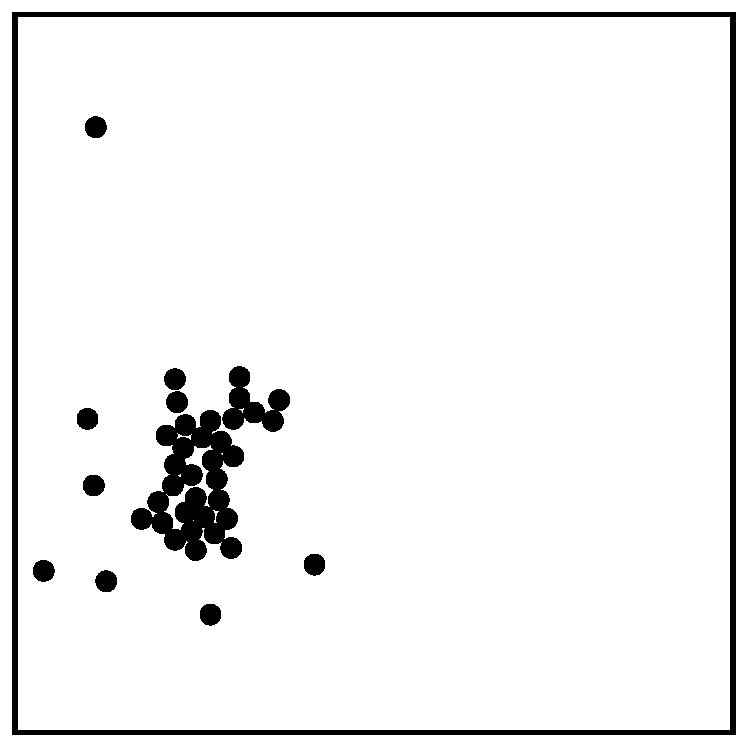
\includegraphics[width=0.6\textwidth]{p1_cold.pdf}
	\end{center}
	\caption{A system of 80 molecules where initially $\frac{E}{N} = -1.2$: Most remain clustered together after thermalization.}
\label{fig:qual}
\end{figure}
\FloatBarrier

\begin{figure}[!htb]
	\begin{center}
		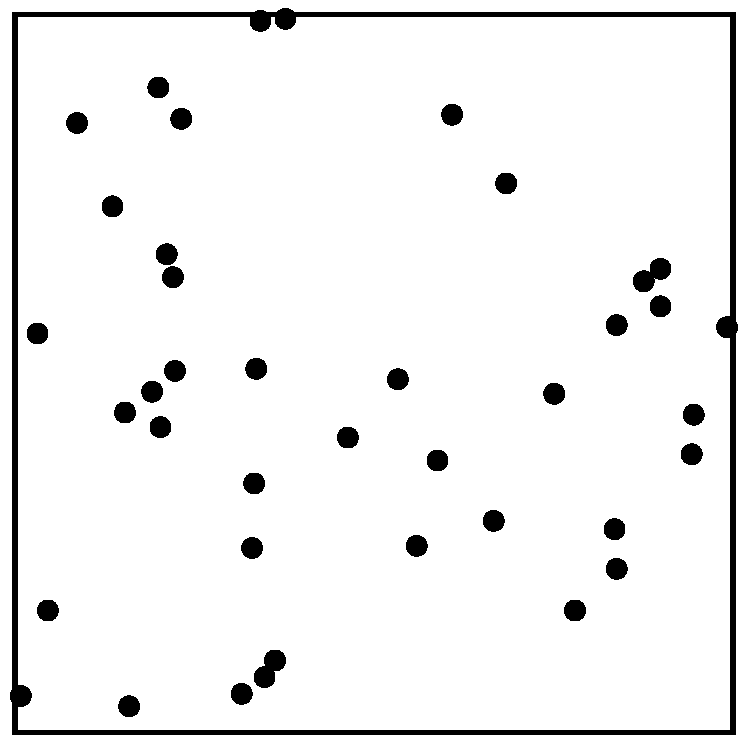
\includegraphics[width=0.6\textwidth]{p1_hot.pdf}
	\end{center}
	\caption{A system of 80 molecules where initially $\frac{E}{N} = 4$: The molecules rapidly escape the potential wells of the other molecules.}
\label{fig:qual}
\end{figure}
\FloatBarrier

\subsection{Question 2}

\begin{figure}[!htb]
	\begin{center}
		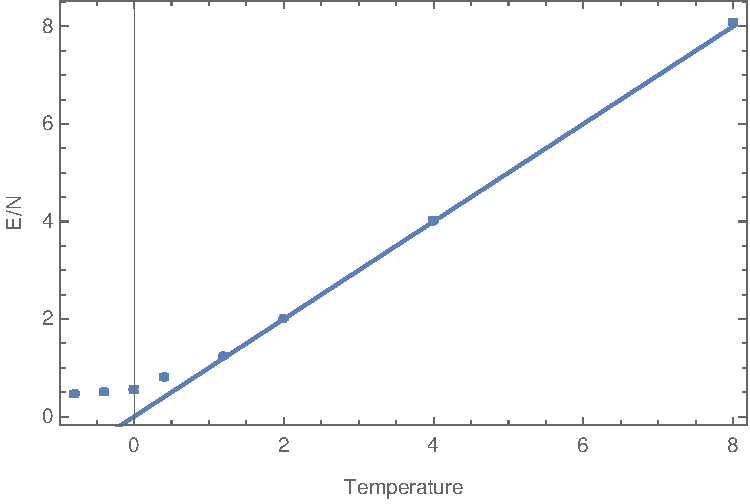
\includegraphics[width=0.6\textwidth]{p2a.pdf}
	\end{center}
	\caption{The E/N vs Temperature of the simulation (points) and the Ideal Gas Law (L = 20)}
\label{fig:qual}
\end{figure}
\FloatBarrier

\begin{figure}[!htb]
	\begin{center}
		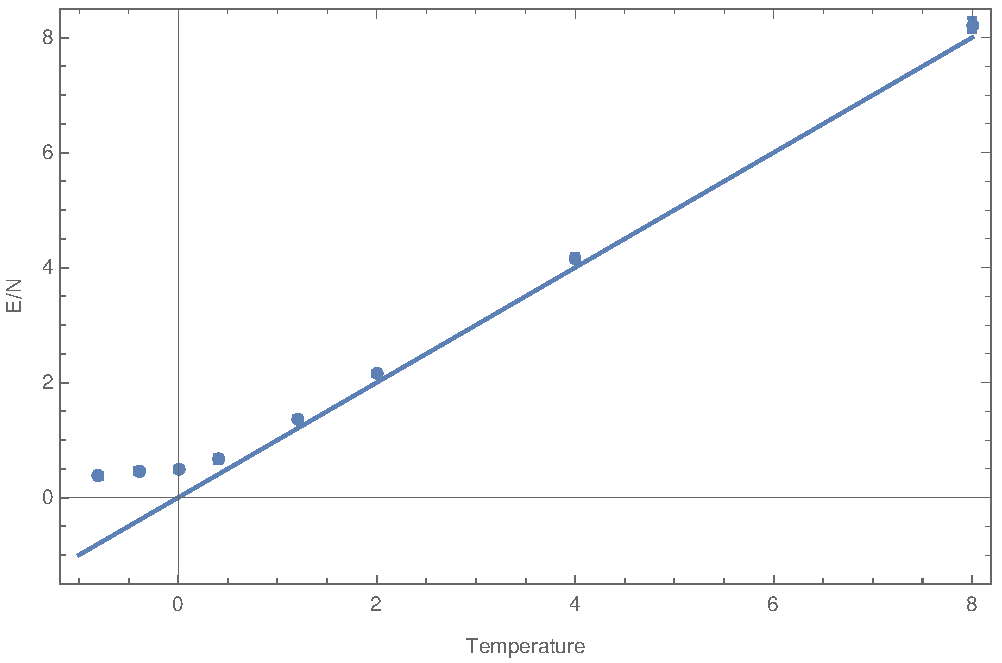
\includegraphics[width=0.6\textwidth]{p2b.pdf}
	\end{center}
	\caption{The E/N vs Temperature of the simulation (points) and the Ideal Gas Law L=16}
\label{fig:qual}
\end{figure}
\FloatBarrier

The size of the box had little effect on the accuracy of the Ideal Gas Law, with major deviation occurring only after the temp drops below 1.7 for both L $ = 20$ and L  $= 16$

\subsection{Question 3}

We see close agreement between the predicted and the observed in the following graphs, though the -0.8 system has a negative skew. I believe that to be an artifact from the system rebounding off of the wall, causing a bulk movement of condensed particles.

\begin{figure}[!htb]
	\begin{center}
		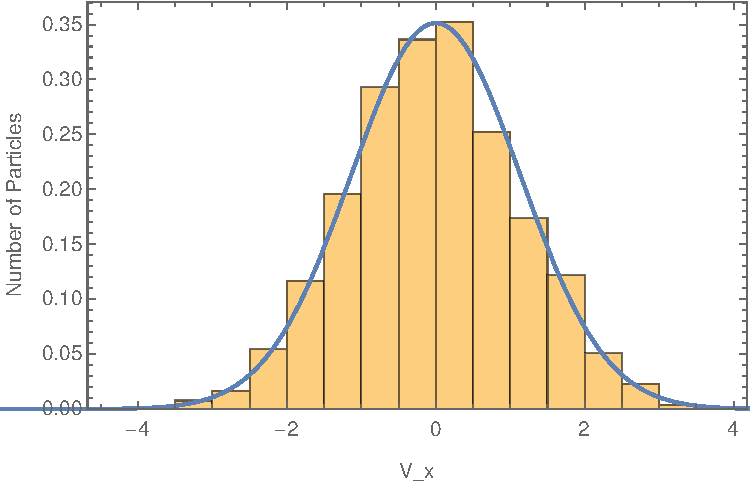
\includegraphics[width=0.6\textwidth]{p3a.pdf}
	\end{center}
	\caption{$\frac{E}{N=1.2}$The Histogram represents the fraction of particles found at various speeds, while the line represents the predicted value}
\label{fig:qual}
\end{figure}
\FloatBarrier

\begin{figure}[!htb]
	\begin{center}
		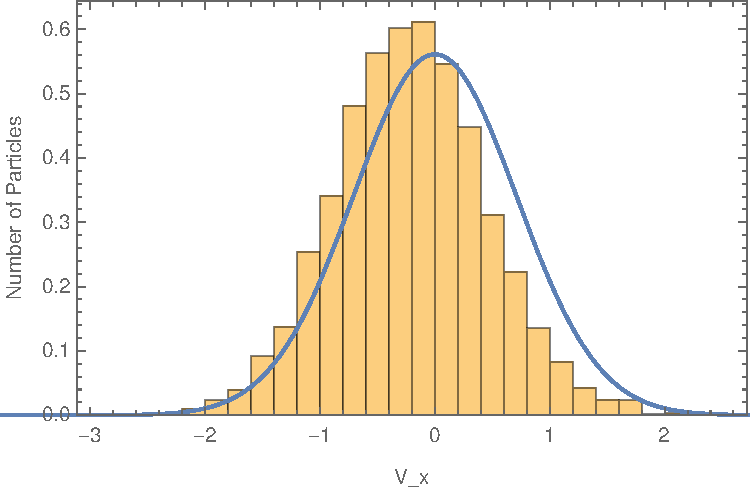
\includegraphics[width=0.6\textwidth]{p3b.pdf}
	\end{center}
	\caption{$\frac{E}{N} = -0.8$The Histogram represents the fraction of particles found at various speeds, while the line represents the predicted value}
\label{fig:qual}
\end{figure}
\FloatBarrier


\subsection{Question 4}

Very close agreement between the Observed and Theoretical models for Pressure.

\begin{figure}[!htb]
	\begin{center}
		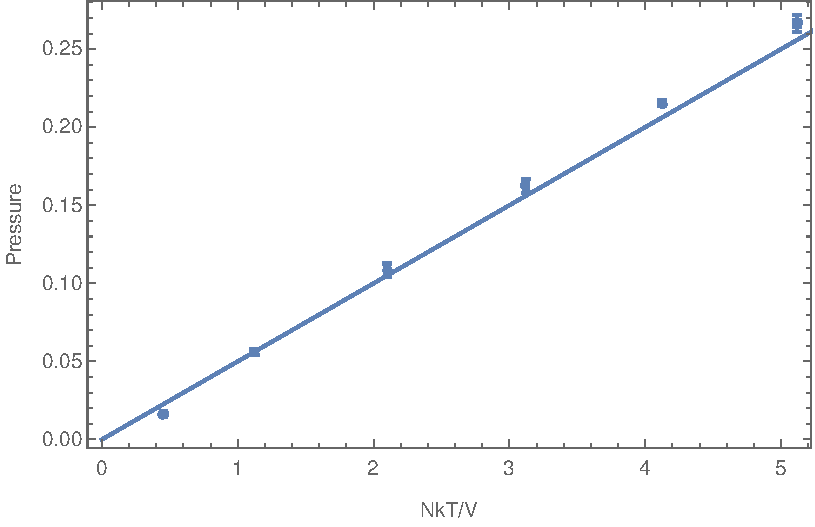
\includegraphics[width=0.6\textwidth]{p4.pdf}
	\end{center}
	\caption{$\frac{E}{N} = -0.8$The Histogram represents the fraction of particles found at various speeds, while the line represents the predicted value}
\label{fig:qual}
\end{figure}
\FloatBarrier






\section{Conclusion}

Monte Carlo simulations are useful windows into understanding bulk properties of fluids.

\end{document}

